\documentclass[
        oneside,      %%coloque  % no in\'icio desta linha para imprimir frente e verso 
        english,			
%	french,				
%	spanish, 
        brazil			 
        ]{abntbibufjf}


\usepackage[T1]{fontenc}		
\usepackage[utf8]{inputenc}		%% Para converter automaticamente acentos como digitados normalmente no teclado. Mude utf8 para latin1 se precisar. 

\usepackage{lmodern} %no caso do modelo Latex, pode-se usar a fam\'ilia de fontes lmodern como aqui indicado, no lugar de Arial e Times New Roman.


\usepackage{lastpage}			
\usepackage{indentfirst}		
\usepackage{color}			
\usepackage{graphicx}			
\usepackage{microtype} 
\usepackage{hyperref}
\usepackage{xurl}
\usepackage{amssymb}
\usepackage{placeins}
% --- Matemática (necessário para \text, \operatorname, \lVert, etc.)
\usepackage{amsmath}
\usepackage{amssymb}
\usepackage{amsfonts}
\usepackage{float}
\usepackage{listings}
\usepackage{xcolor}


% Configuração do estilo para Python
\lstset{
  language=Python,
  basicstyle=\ttfamily\small,
  keywordstyle=\color{blue},
  stringstyle=\color{red!70!black},
  commentstyle=\color{green!50!black}\itshape,
  numberstyle=\tiny\color{gray},
  numbers=left,
  stepnumber=1,
  numbersep=8pt,
  backgroundcolor=\color{gray!10},
  frame=single,
  tabsize=4,
  showstringspaces=false,
  breaklines=true,
  captionpos=b
}

%% -----------------------------------------------------------------------------

%% Obs.: Alguns acentos foram omitidos.

\titulo{Identificação do Ideal Customer Profile em Negócios B2B} 
\subtitulo{Modelo Computacional Aplicado ao Setor de Benefícios Corporativos}  %% Colocar % no in\'icio desta linha se nao tiver subt\'itulo 
\autor{Félix Oliveira Miranda} %%Colocar, dentro de chaves {}, o nome completo do autor
\autorVirg{Miranda, Félix Oliveira} %%Colocar o sobrenome do autor, separado por v\'rgula, antes do restante do nome do autor. Ex.: Santos, Maria dos
\local{Juiz de Fora} %%Governador Valadares % N\~ao usar MG.
\data{2025} %%Colocar o ano da entrega. Por exemplo, 2019. N\~ao usar m\^es.
\orientador[Orientadora:]{Priscila Vanessa Zabala Capriles Golliat} %%Se precisar, troque [Orientador:] por [Orientadora:]
%\coorientador[Coorientador:]{Nome e sobrenome} %% Colocar ``%'' no in\'icio desta linha se n\~ao tiver coorientador. Se precisar, troque por [Cooorientadora:]. 
\orientadorTitulo{Profa. Dra.} %%Colocar, dentro de chaves {}, a titula\c{c}\~ao do(a) orientador(a). Por exemplo, Prof. Dr.
%\coorientadorTitulo{Titula\c{c}\~ao} %%Colocar, dentro de chaves {}, a titula\c{c}\~ao do(a) cooorientador(a). 
\instituicao{Universidade Federal de Juiz de Fora}
\faculdade{Faculdade de Engenharia} %%Colocar, dentro de chaves {}, o nome da faculdade ou do instituto.
\programa{Engenharia Computacional} %%Colocar, dentro de chaves {}, o nome do curso. Por exemplo: Programa de P\'os\mbox{-Gra}dua\c{c}\~ao em Matem\'atica
\objeto{Trabalho de Conclusão de Curso (graduação)}  %%Tese (Doutorado)  %%%Trabalho de Conclus\~ao de Curso (gradua\c{c}\~ao)
\natureza{Trabalho de conclusão de curso apresentado à \inserefaculdade~da
Universidade Federal de Juiz de Fora como requisito parcial à obtenção do
grau de Bacharel em Engenharia Computacional.}

%% Abaixo, prencher com os dados da parte final da ficha catalografica
\finalcatalog{1. Palavra-chave. 2. Palavra-chave. 3. Palavra-chave. I. Sobrenome, Nome do orientador, orient. II. T\'itulo.} %% Aqui fica 
% escrito a palavra ``T\'itulo'' mesmo, nao o do trabalho. Se tiver coorientador, os dados ficam depois dos dados 
%% do orientador (II. Sobrenome, Nome do coorientador, coorient.) e antes de ``II. T\'itulo'', o qual passa a ``III. T\'itulo''.


%\usepackage[round, numbers]{natbib} %para refer\^encias bibliogr\'aficas no sistema num\'erico com () na chamada da citacao. 

%Se for usar o sistema autor-data, colocar % antes de \usepackage acima e retirar % antes de \usepackage abaixo.

\usepackage{natbib} %para o sistema autor-data

\begin{document}

%% ELEMENTOS PR\'E-TEXTUAIS


%% Capa. N\~ao entra na contagem da pagina\c{c}\~ao.
\inserecapa

%% Folha de rosto
\inserefolhaderosto

%% Ficha catalogr\'afica. AO IMPRIMIR, DEIXAR NO VERSO DA FOLHA DE ROSTO.
\inserecatalog  


%% Folha de aprovacao. Incluir mesmo que sem assinaturas. Assinaturas eletr\^onicas via SEI.
\begin{folhadeaprovacao}
\inicfolhaaprov
        
Aprovada em (dia) de (m\^es) de (ano) %%Preencher com a data 
   
\vfill
\begin{center} BANCA EXAMINADORA \end{center}
\assinatura{\insereorientadorTitulo~\insereorientador \ - Orientador \\ Universidade Federal de Juiz de Fora}  %%Orientadora
%\assinatura{Professor Dr. \inserecoorientador \ - Coorientador \\ Universidade Federal de Juiz de Fora}
\assinatura{Titula\c{c}\~ao Nome e sobrenome \\ Universidade ???}
\assinatura{Titula\c{c}\~ao Nome e sobrenome  \\ Universidade ??} 
%\assinatura{...} %%RETIRE O % E PREENCHA SE PRECISAR
%  \assinatura{...}
%  \assinatura{...}
\end{folhadeaprovacao}
\cleardoublepage 

 
%% Agradecimentos. OPCIONAL. Caso seja bolsista, inserir os devidos agradecimentos.
\begin{agradecimentos}

Agradeço, em primeiro lugar, ao meu pai, \textbf{Félix de Valois}, o maior investidor e incentivador desta jornada. Foi ele quem acreditou em mim desde o primeiro momento, quem cobrou, orientou e fomentou cada etapa da minha formação. Todo este percurso só foi possível graças ao seu esforço, confiança e presença constante. Principalmente por ter me feito seguir caminhos que eu só compreenderia posteriomente na vida, e que hoje sou eternamente grato a ele.

À minha mãe, \textbf{Izabel Maria}, por nunca ter medido esforços para que eu tivesse tudo de que precisasse. É somente por causa dela que cheguei até a Universidade Federal de Juiz de Fora, e tudo o que ela enfrentou para me ver aqui é motivo de profunda admiração e gratidão.  

À minha irmã, \textbf{Isabella}, pelo carinho e pela torcida incondicional.  

Ao meu tio, \textbf{João Filho}, que me acompanhou no início da minha trajetória e me deu o apoio necessário para dar os primeiros passos no começo da trajetória acadêmica.  

À minha namorada, \textbf{Gabriella}, um verdadeiro farol de luz na minha vida. Obrigado por sempre me colocar para cima, acreditar em mim e ser uma mulher incrível neste fechamento de ciclo. Sua presença foi essencial para que eu seguisse firme até o fim.  

Estendo meus agradecimentos também a três professores que marcaram profundamente minha formação. Ao \textbf{Professor Leonardo Golliat} e à \textbf{Professora Priscila Capriles}, pela oportunidade transformadora de atuar no projeto da ArcelorMittal, onde pude construir as bases do profissional de dados que sou hoje. E à \textbf{Professora Ana Sophia Cavalcanti}, por compartilhar comigo tantas conquistas, pela parceria e incentivo constante ao longo da nossa jornada na capitania da equipe Rinobot.  

A todos vocês, meu sincero agradecimento por acreditarem em mim, mesmo quando eu duvidei. Este trabalho é, acima de tudo, o reflexo de tudo que aprendi e vivi ao lado de vocês.

\end{agradecimentos}

%% RESUMOS

%% Resumo em Portugu\^es. OBRIGAT\'ORIO. \'E obrigat\'orio o uso de par\'agrafo \'unico.
\begin{resumo}

  Este trabalho tem como objetivo desenvolver um modelo computacional para a identificação do Ideal Customer Profile (ICP) em negócios B2B (business-to-business), ou seja, relações comerciais estabelecidas entre empresas, com foco em fornecedores de benefícios corporativos como Unimed, Swile e TotalPass. Para isso, foi estruturada uma pipeline de aquisição e enriquecimento de dados baseada em técnicas de web scraping, consumo de APIs públicas e firmográficas, e normalização por CNPJ. A metodologia adota uma abordagem híbrida, combinando One-Class Classification (OCC), utilizada para filtrar empresas fora do perfil desejado, com Distance-Based Scoring (DBS), responsável por ranquear os leads restantes de acordo com sua similaridade com o ICP. O processo inclui ainda etapas de pré-processamento, padronização de variáveis contínuas e one-hot encoding de variáveis categóricas, resultando em uma base vetorizada adequada para a modelagem. Espera-se que os resultados obtidos contribuam para a definição de clientes ideais em ambientes B2B complexos, permitindo maior assertividade na priorização de leads, otimização de recursos de vendas e marketing, e geração de insights para estratégias comerciais, além de apontar caminhos futuros para aprimoramento metodológico, como o uso de aprendizado profundo e integração com sistemas CRM em produção.

  Palavras-chave: Ideal Customer Profile; ICP; Business-to-Business; OCC; DBS.
  
  \end{resumo}
 
 
%% Resumo em Ingl\^es. \'E obrigat\'orio o uso de par\'agrafo \'unico.
\begin{resumo}[ABSTRACT]
  \begin{otherlanguage*}{english}

  This work aims to develop a computational model for identifying the Ideal Customer Profile (ICP) in B2B (business-to-business) contexts, that is, commercial relationships established between companies, with a specific focus on corporate benefits providers such as Unimed, Swile, and TotalPass. A data acquisition and enrichment pipeline was designed, combining web scraping techniques, consumption of public and firmographic APIs, and normalization through the Brazilian corporate tax ID (CNPJ). The methodology adopts a hybrid approach, combining One-Class Classification (OCC), used to filter out companies outside the desired profile, with Distance-Based Scoring (DBS), responsible for ranking the remaining leads according to their similarity to the ICP. The process also includes preprocessing steps such as standardization of continuous variables and one-hot encoding of categorical variables, resulting in a vectorized dataset suitable for modeling. The expected outcome is to contribute to the definition of ideal customers in complex B2B environments, enabling greater accuracy in lead prioritization, optimization of sales and marketing resources, and generation of insights for business strategies, while also pointing to future directions such as the use of deep learning techniques and integration with production CRM systems. \\[18pt]

  Keywords: Ideal Customer Profile; ICP; Business-to-Business; OCC; DBS.

  \end{otherlanguage*}
\end{resumo}

\pdfbookmark[0]{\listfigurename}{lof}

%Caso as ilustra\c{c}~oes do trabalho sejam todas do mesmo tipo (por exemplo, todas do tipo organograma), coloque % no in\'icio das duas linhas abaixo. 
\ilustvaria   %Use este comando somente caso as ilustra\c{c}\~oes n\~ao sejam todas do mesmo tipo. 
\listilustvaria  %Use este comando somente caso as ilustra\c{c}\~oes n\~ao sejam todas do mesmo tipo e caso queira inserir a lista delas. 

%\listoffigures*  %Use este comando quando todas as ilustra\c{c}\~oes s\~ao do mesmo tipo e caso queira inserir a lista delas. Veja dicas no final deste arquivo.

\cleardoublepage
\pdfbookmark[0]{\listtablename}{lot}

%% Lista de tabelas. OPCIONAL. A ordem da lista de tabelas deve obrigatoriamente ser a mesma ordem em que as tabelas aparecem no texto. 


\listoftables*    %Coloque ``%'' no in\'icio desta linha, caso n\~ao queira lista de tabelas. 

\cleardoublepage

%% Lista de abreviaturas e siglas. OPCIONAL. Nao deve haver sinal grafico entre as siglas e abreviaturas e o significado. 

\begin{siglas}

  \item[ABNT] Associa\c{c}\~ao Brasileira de Normas T\'ecnicas
  \item[API] Application Programming Interface (Interface de Programa\c{c}\~ao de Aplica\c{c}\~oes)
  \item[B2B] Business-to-Business (Neg\'ocios entre Empresas)
  \item[CAC] Custo de Aquisi\c{c}\~ao de Cliente
  \item[CNAE] Classifica\c{c}\~ao Nacional de Atividades Econ\^omicas
  \item[CNPJ] Cadastro Nacional da Pessoa Jur\'idica
  \item[CRM] Customer Relationship Management (Gest\~ao de Relacionamento com o Cliente)
  \item[DBS] Distance-Based Scoring
  \item[IBGE] Instituto Brasileiro de Geografia e Estat\'istica
  \item[ICP] Ideal Customer Profile (Perfil Ideal de Cliente)
  \item[IF] Isolation Forest
  \item[LGPD] Lei Geral de Prote\c{c}\~ao de Dados
  \item[LTV] Lifetime Value (Valor do Ciclo de Vida do Cliente)
  \item[OCC] One-Class Classification
  \item[OHE] One-Hot Encoding
  \item[TI] Tecnologia da Informa\c{c}\~ao
  \item[UF] Unidade Federativa

\end{siglas}
 
%% Sum\'ario

\pdfbookmark[0]{\contentsname}{toc}
\tableofcontents*
\cleardoublepage

%% ----------------------------------------------------------

%% ELEMENTOS TEXTUAIS
\textual

\include{capitulos/Introdução}

\include{capitulos/Fundamentação Teórica}

\include{capitulos/Trabalhos Relacionados}

\include{capitulos/Aquisição e Tratamento dos Dados}

\include{capitulos/Construção do Modelo Computacional}

\chapter{RESULTADOS}

\noindent
Este capítulo apresenta os resultados empíricos obtidos a partir da aplicação do modelo híbrido (OCC + DBS) para a base de clientes das cinco corporações analisadas: Gympass, Totalpass, Swile, Unimed e Psicologia Viva.


\section{Visão Geral do Pré-Processamento das Bases}

O pré-processamento foi conduzido de forma padronizada para todas as bases analisadas, assegurando comparabilidade entre os provedores de benefícios corporativos. Em ambas as bases — TotalPass, Gympass, Swile, Unimed e Psicologia Viva — foram aplicadas etapas de limpeza, renomeação, remoção de colunas irrelevantes, separação da variável \textit{localização} em \textit{cidade} e \textit{estado}, e vetorização numérica das variáveis firmográficas.

A Tabela~\ref{tab:7_1_pre_all} apresenta o resumo das principais características de pré-processamento para as cinco empresas analisadas até o momento. Nota-se que as estruturas são semelhantes, variando apenas no número de observações e colunas finais após codificação vetorial.

\begin{table}[H]
\centering
\caption{Resumo comparativo do pré-processamento das bases.}
\label{tab:7_1_pre_all}
\begin{tabular}{lcccc}
\toprule
\textbf{Provedor} & \textbf{Empresas} & \textbf{Variáveis Vetorizadas} & \textbf{Numéricas} & \textbf{Categóricas} \\
\midrule
Gympass & 251 & 145 & capital\_social, funcionários & estado, segmento \\
Psicologia Viva & 187 & 122 & capital\_social, funcionários & estado, segmento \\
Swile & 281 & 139 & capital\_social, funcionários & estado, segmento \\
TotalPass & 351 & 202 & capital\_social, funcionários & estado, segmento \\
Unimed & 338 & 198 & capital\_social, funcionários & estado, segmento \\
\bottomrule
\end{tabular}
\end{table}

A uniformidade metodológica garante que as diferenças observadas nos resultados posteriores sejam reflexo das características reais das empresas de cada base, e não de inconsistências de pré-processamento. As pequenas variações no número de variáveis decorrem de diferenças na cardinalidade dos segmentos e estados representados.

\section{Análise Exploratória das Bases}

A análise exploratória teve como objetivo compreender a composição e dispersão dos dados após o pré-processamento, verificando padrões geográficos, setoriais e de porte entre as empresas de cada base.

\subsection{Distribuição Geográfica}

A Figura~\ref{fig:map} apresentará a distribuição por estado das empresas das cinco bases. Em todas, o estado de São Paulo concentra a maioria absoluta das empresas — 184 (52\%) no TotalPass e 72 (29\%) no Gympass — seguido por presenças menores em Rio de Janeiro, Minas Gerais, Paraná e Santa Catarina. Esse padrão reflete a centralização econômica e tecnológica na região Sudeste.

\begin{figure}[H]
    \centering
    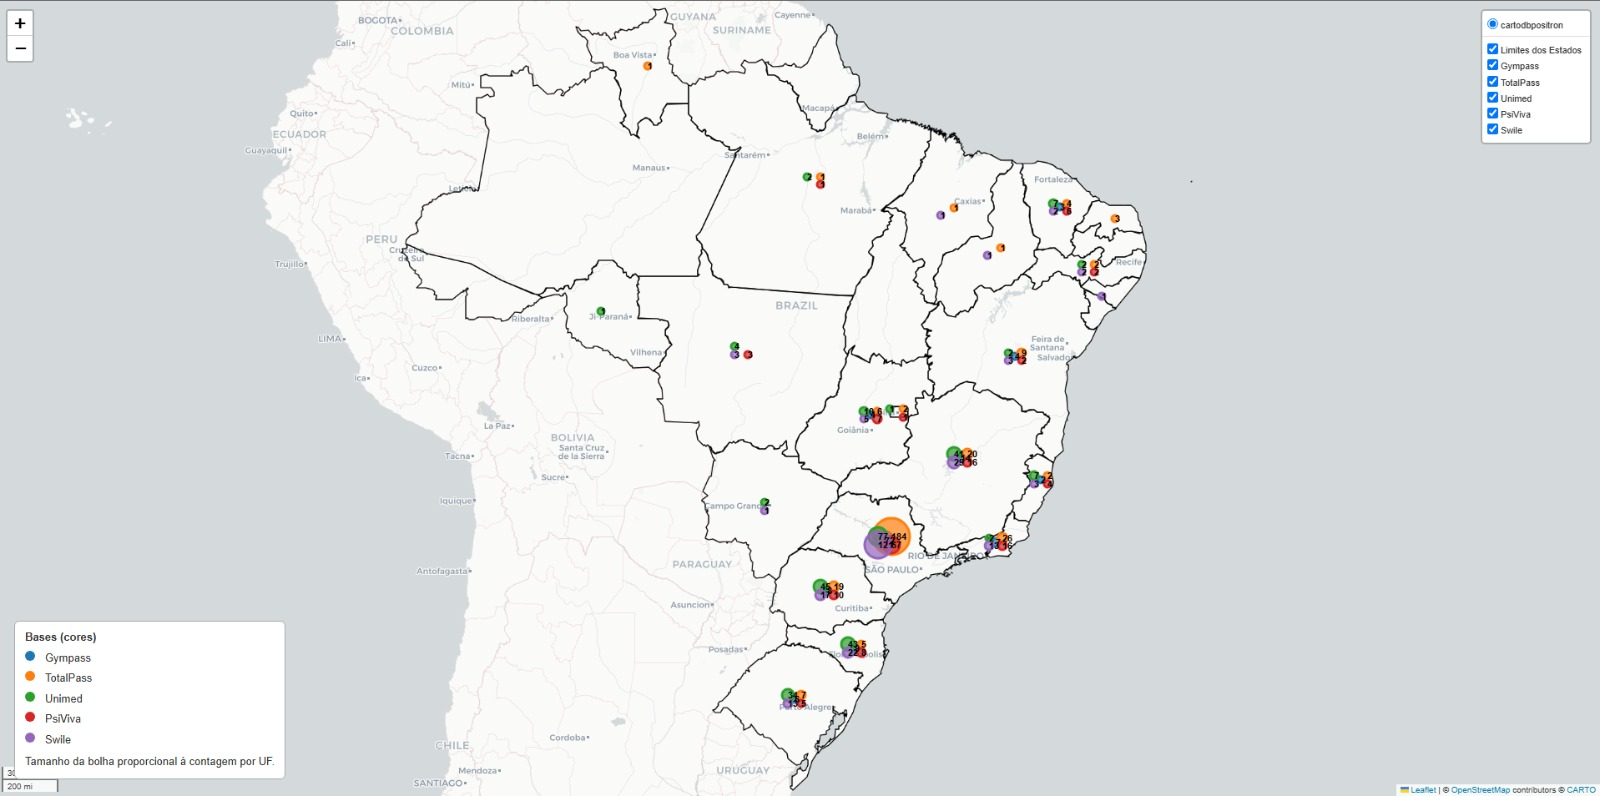
\includegraphics[width=0.9\textwidth]{imagens/Map.jpeg}
    \caption{Distribuição geográfica por UF — mapa consolidado das cinco bases.}
    \label{fig:map}
    \legend{Fonte: elaboração própria.}
\end{figure}

\subsection{Distribuição por Segmento}

As cinco bases exibem predominância de setores ligados à tecnologia e serviços corporativos. No TotalPass, destacam-se \textit{Desenvolvimento de programas de computador sob encomenda} e \textit{Consultoria em TI}; já no Gympass, sobressaem \textit{Desenvolvimento e licenciamento de softwares customizáveis} e \textit{Holdings de instituições não-financeiras}. Essa consistência indica que o modelo de benefícios corporativos tende a atrair empresas com perfis digitais ou administrativos.

\subsection{Estatísticas Descritivas}

A Tabela~\ref{tab:7_3a_capital} sintetiza as estatísticas de \textit{capital\_social} enquanto a Tabela~\ref{tab:7_3b_funcionarios} apresenta as estatísticas de \textit{funcionários}. Observa-se ampla dispersão, típica de bases heterogêneas compostas por empresas de portes distintos. A mediana e o intervalo interquartil, contudo, indicam predominância de empresas de médio porte.

\begin{table}[H]
\centering
\caption{Estatísticas descritivas de \textit{Capital Social} por provedor.}
\label{tab:7_3a_capital}
\begin{tabular}{lrrrr}
\toprule
\textbf{Provedor} & \textbf{Média (R\$)} & \textbf{Mediana (R\$)} & \textbf{Mínimo} & \textbf{Máximo} \\
\midrule
TotalPass & 8,79e+08 & 6,73e+06 & 0 & 7,04e+10 \\
Gympass & 1,62e+09 & 3,30e+07 & 0 & 9,07e+10 \\
Swile & 5,39e+07 & 4,65e+05 & 0 & 2,77e+09 \\
Unimed & 2,24e+08 & 1,00e+06 & 0 & 2,43e+10 \\
Psicologia Viva & 1,16e+09 & 4,60e+05 & 0 & 8,71e+10 \\
\bottomrule
\end{tabular}
\end{table}

\begin{table}[H]
\centering
\caption{Estatísticas descritivas de \textit{Número de Funcionários} por provedor.}
\label{tab:7_3b_funcionarios}
\begin{tabular}{lrrrr}
\toprule
\textbf{Provedor} & \textbf{Média} & \textbf{Mediana} & \textbf{Mínimo} & \textbf{Máximo} \\
\midrule
TotalPass & 3.022 & 323 & 1 & 111.275 \\
Gympass & 12.815 & 432 & 1 & 670.501 \\
Swile & 735 & 95 & 1 & 44.770 \\
Unimed & 1.812 & 196 & 1 & 79.911 \\
Psicologia Viva & 7.659 & 254 & 1 & 366.668 \\
\bottomrule
\end{tabular}
\end{table}

Ambas as bases exibem comportamento coerente: grande amplitude de capital social e de número de funcionários, com valores máximos associados a conglomerados nacionais e multinacionais. Essa variação reforça a importância da etapa de filtragem de anomalias apresentada na seção seguinte.

% Inserir Figura 7.1 — Distribuição por estado (comparativa)
% Inserir Figura 7.2 — Distribuição por segmento (comparativa)

% --- Filtro de Anomalias (OCC — Isolation Forest) ---
\section{Filtro de Anomalias (OCC — Isolation Forest)}

A detecção de anomalias foi conduzida por meio de um único modelo OCC (\textit{One-Class Classification}), o \textit{Isolation Forest}. O objetivo foi identificar empresas fora do perfil padrão de cliente ideal (ICP) e delimitar o conjunto de \textit{inliers} que serviriam como base para o cálculo do \textit{Distance-Based Scoring} (DBS).

A Tabela~\ref{tab:7_4_occ_all} apresenta o resumo comparativo dos resultados do \textit{Isolation Forest} aplicado às bases TotalPass, Gympass, Swile, Unimed e Psicologia Viva. Em todos os casos, observou-se baixo percentual de anomalias e valores de score médio positivos e próximos de zero, indicando estabilidade e ausência de distorções.

\begin{table}[H]
\centering
\caption{Resumo comparativo do filtro de anomalias via Isolation Forest.}
\label{tab:7_4_occ_all}
\begin{tabular}{lrrrrr}
\toprule
\textbf{Provedor} & \textbf{Empresas Totais} & \textbf{Anomalias} & \textbf{\% Outliers} & \textbf{Score Médio} & \textbf{Faixa de Scores} \\
\midrule
Gympass & 251 & 13 & 5,2\% & 0,0163 & [-0,0264 ; 0,0319] \\
Psicologia Viva & 187 & 10 & 5,3\% & 0,0156 & [-0,0115 ; 0,0323] \\
Swile & 281 & 14 & 5,0\% & 0,0165 & [-0,0144 ; 0,0326] \\
TotalPass & 351 & 18 & 5,1\% & 0,0187 & [-0,0119 ; 0,0338] \\
Unimed & 338 & 17 & 5,0\% & 0,0124 & [-0,0151 ; 0,0243] \\
\bottomrule
\end{tabular}
\end{table}


Os resultados demonstram consistência no comportamento do modelo, com proporções similares de anomalias nas cinco bases. Essa estabilidade reforça a adequação do \textit{Isolation Forest} como ferramenta de filtragem prévia para a metodologia proposta.

As Figuras abaixo mostram a distribuição dos scores de anomalia para todas as bases, evidenciando que a maior parte das empresas apresenta valores próximos à faixa neutra (entre 0,01 e 0,03), indicando alinhamento ao perfil ICP.

\begin{figure}[H]
    \centering
    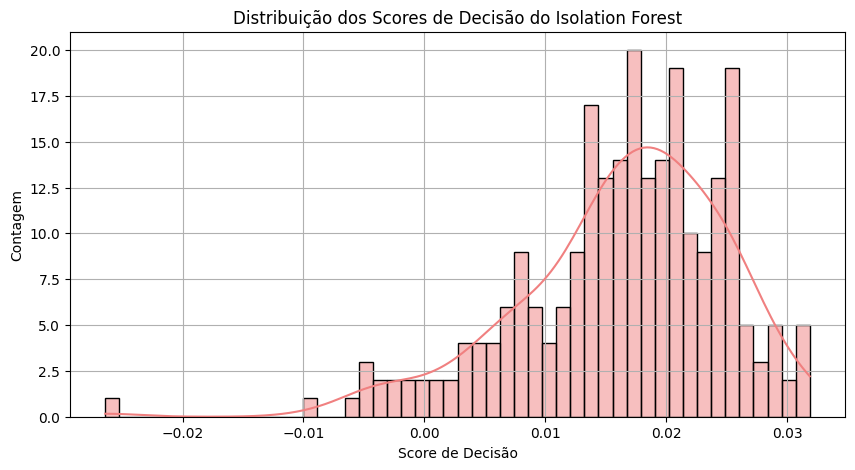
\includegraphics[width=0.9\textwidth]{imagens/gympass_iso_forest.png}
    \caption{Distribuição dos Scores de Decisão do modelo Isolation Forest — Gympass.}
    \label{fig:gympass_iso_forest}
    \legend{Fonte: elaboração própria.}
\end{figure}

\begin{figure}[H]
    \centering
    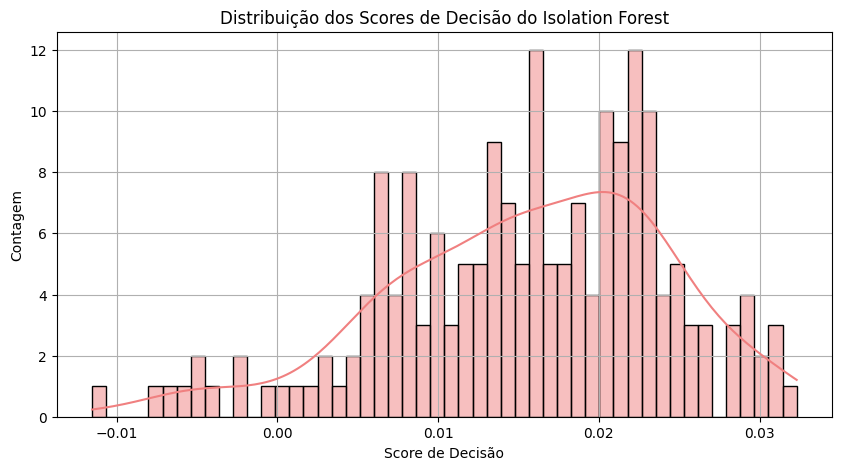
\includegraphics[width=0.9\textwidth]{imagens/psiviva_iso_forest.png}
    \caption{Distribuição dos Scores de Decisão do modelo Isolation Forest — Psicologia Viva.}
    \label{fig:psiviva_iso_forest}
    \legend{Fonte: elaboração própria.}
\end{figure}

\begin{figure}[H]
    \centering
    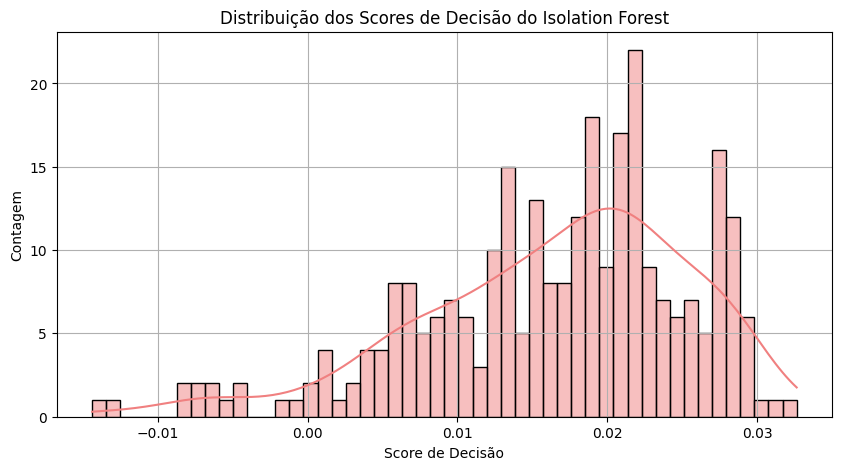
\includegraphics[width=0.9\textwidth]{imagens/swile_iso_forest.png}
    \caption{Distribuição dos Scores de Decisão do modelo Isolation Forest — Swile.}
    \label{fig:swile_iso_forest}
    \legend{Fonte: elaboração própria.}
\end{figure}

\begin{figure}[H]
    \centering
    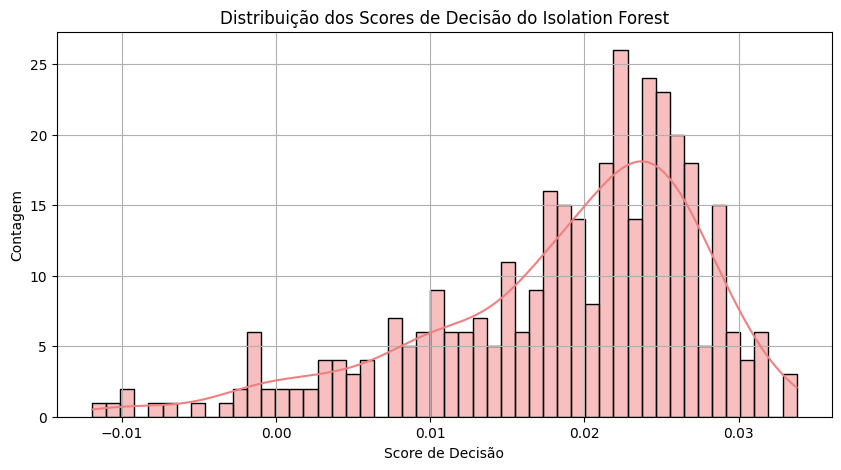
\includegraphics[width=0.9\textwidth]{imagens/totalpass_iso_forest.png}
    \caption{Distribuição dos Scores de Decisão do modelo Isolation Forest — TotalPass.}
    \label{fig:totalpass_iso_forest}
    \legend{Fonte: elaboração própria.}
\end{figure}

\begin{figure}[H]
    \centering
    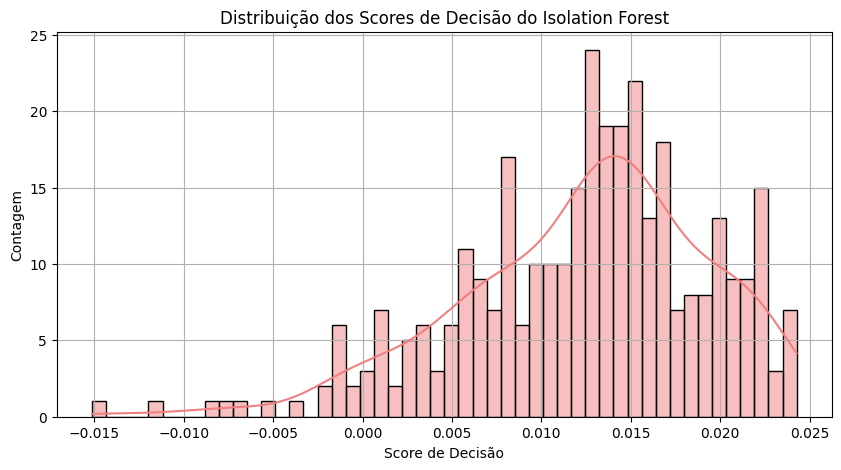
\includegraphics[width=0.9\textwidth]{imagens/unimed_iso_forest.png}
    \caption{Distribuição dos Scores de Decisão do modelo Isolation Forest — Unimed.}
    \label{fig:unimed_iso_forest}
    \legend{Fonte: elaboração própria.}
\end{figure}

% Inserir Boxplot 7.4 — Comparação da proporção de outliers entre bases

Em síntese, o filtro OCC apresentou comportamento estável e seletivo, com percentual de anomalias próximo a 5\% em todas as amostras. Essa constância confirma a robustez do método e sua aplicabilidade transversal entre diferentes provedores de benefícios corporativos.

% --- NOVA SEÇÃO: Modelagem Distance-Based Scoring (DBS) ---

\section{Modelagem Distance-Based Scoring (DBS)}

Após a filtragem das anomalias, as empresas classificadas como \textit{inliers} pelo \textit{Isolation Forest} foram submetidas à etapa de modelagem por distância (\textit{Distance-Based Scoring} — DBS). Essa abordagem permitiu quantificar o grau de similaridade de cada empresa ao perfil médio de cliente ideal (ICP), utilizando duas métricas complementares: \textit{distância ao centróide} e \textit{distância média aos dez vizinhos mais próximos} (\textit{k}-NN).

A Tabela~\ref{tab:7_5_dbs_all} apresenta o resumo comparativo dos resultados médios obtidos para as cinco bases analisadas até o momento. As médias elevadas e a baixa dispersão confirmam a concentração das empresas em torno de um núcleo firmográfico comum, característica esperada de um conjunto representativo do ICP.

\begin{table}[H]
\centering
\caption{Resumo comparativo dos scores DBS.}
\label{tab:7_5_dbs_all}
\begin{tabular}{lrrrrr}
\toprule
\textbf{Provedor} & \textbf{Empresas (Inliers)} & \textbf{Média Centróide} & \textbf{Desvio-Padrão} & \textbf{Média k-NN} & \textbf{Desvio-Padrão} \\
\midrule
Gympass & 238 & 0,9663 & 0,1054 & 0,8894 & 0,0923 \\
Psicologia Viva & 177 & 0,9698 & 0,1026 & 0,9583 & 0,0993 \\
Swile & 267 & 0,9288 & 0,1119 & 0,7268 & 0,1262 \\
TotalPass & 333 & 0,9628 & 0,0805 & 0,8772 & 0,0729 \\
Unimed & 321 & 0,9788 & 0,0816 & 0,9410 & 0,0701 \\
\bottomrule
\end{tabular}
\end{table}

Os valores próximos entre os cinco provedores demonstram a consistência da metodologia: a variação inferior a 0,01 na média dos scores centróide e k-NN indica comportamento estável, independentemente do tamanho da base ou da natureza das empresas analisadas. 

\subsection{Análise Interpretativa}

O score centróide, associado à similaridade global com o perfil médio, apresentou valores ligeiramente superiores ao k-NN em todas as amostras, o que sugere que o conjunto de empresas tende a formar um núcleo compacto com pequenas variações locais. Essa diferença é desejável, pois o componente k-NN atua como refinamento da análise global, capturando pequenas nuances setoriais e regionais.

\subsection{DBS por Provedor: Centróide e k-NN}

\noindent
Nesta subseção, apresentamos, para cada provedor, (i) o gráfico de distância ao centróide — que resume a similaridade global ao perfil médio de ICP — e (ii) a distribuição dos \textit{scores} via \textit{k}-NN — que refina a análise pela proximidade local no espaço vetorial.

% --- GYMPASS ---
\subsubsection*{Gympass}
\noindent
O centróide do Gympass indica alta coesão em torno do perfil médio (pico próximo a 1,0), enquanto a distribuição do k-NN revela leve assimetria à esquerda, sinalizando subgrupos setoriais com maior densidade.

\begin{figure}[H]
    \centering
    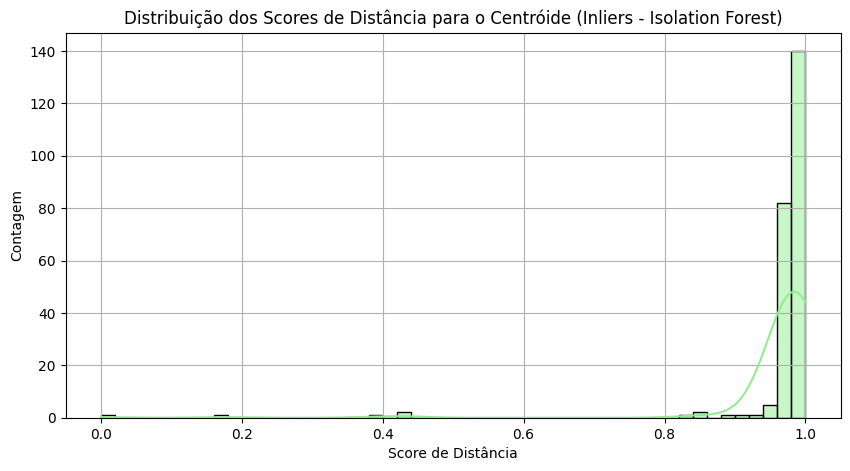
\includegraphics[width=0.9\textwidth]{imagens/gympass_centroid.png}
    \caption{DBS — Distância ao Centróide (Gympass).}
    \label{fig:gympass_centroid}
    \legend{Fonte: elaboração própria.}
\end{figure}

\begin{figure}[H]
    \centering
    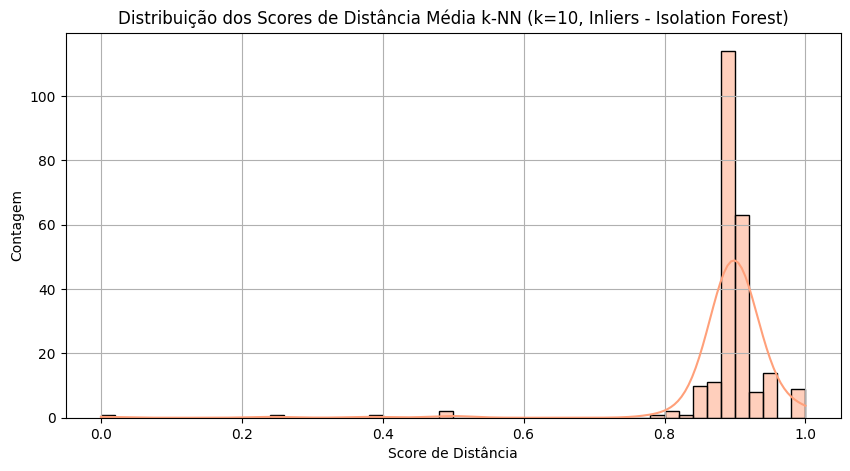
\includegraphics[width=0.9\textwidth]{imagens/gympass_knn.png}
    \caption{DBS — Distribuição de Scores k-NN (Gympass).}
    \label{fig:gympass_knn}
    \legend{Fonte: elaboração própria.}
\end{figure}

% --- PSICOLOGIA VIVA ---
\subsubsection*{Psicologia Viva}
% \noindent
% Observa-se centróide concentrado em valores elevados (≥0,95), sugerindo forte alinhamento médio ao ICP; a distribuição k-NN mantém patamar alto com cauda curta, indicando baixa heterogeneidade local.

\begin{figure}[H]
    \centering
    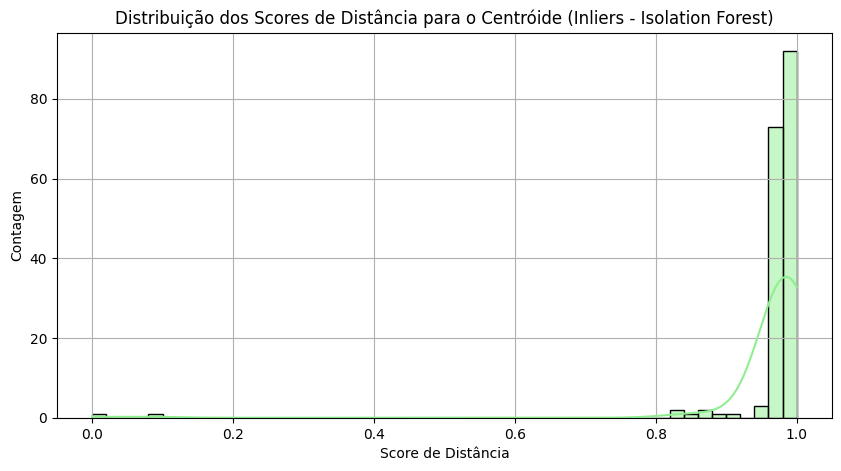
\includegraphics[width=0.9\textwidth]{imagens/psiviva_centroid.png}
    \caption{DBS — Distância ao Centróide (Psicologia Viva).}
    \label{fig:psiviva_centroid}
    \legend{Fonte: elaboração própria.}
\end{figure}

\begin{figure}[H]
    \centering
    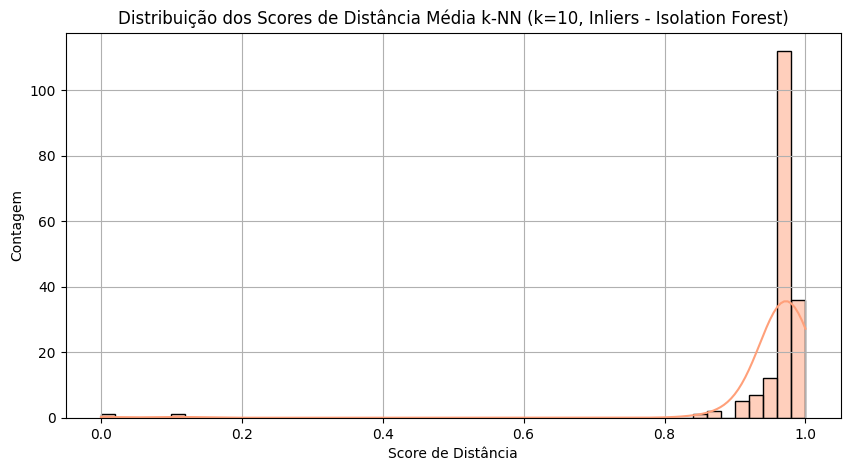
\includegraphics[width=0.9\textwidth]{imagens/psiviva_knn.png}
    \caption{DBS — Distribuição de Scores k-NN (Psicologia Viva).}
    \label{fig:psiviva_knn}
    \legend{Fonte: elaboração própria.}
\end{figure}

% --- SWILE ---
\subsubsection*{Swile}
\noindent
A distância ao centróide apresenta ligeira dispersão comparada aos demais provedores, sugerindo maior variedade firmográfica; o k-NN evidencia \textit{clusters} locais mais pronunciados, úteis para segmentação fina.

\begin{figure}[H]
    \centering
    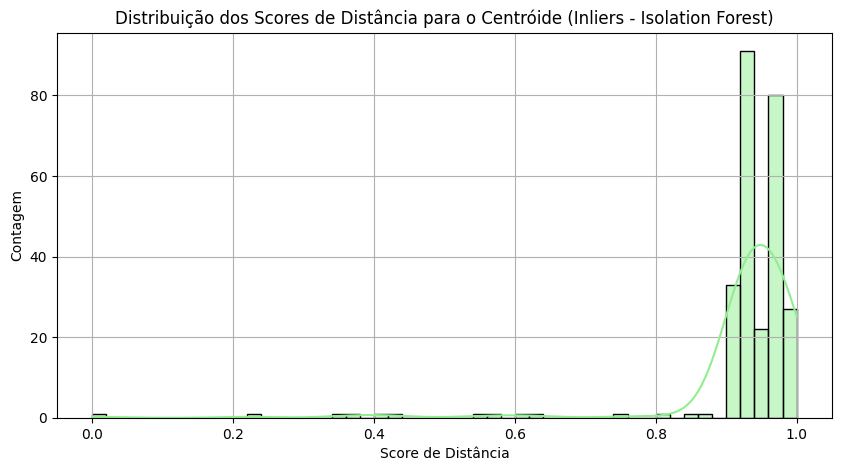
\includegraphics[width=0.9\textwidth]{imagens/swile_centroid.png}
    \caption{DBS — Distância ao Centróide (Swile).}
    \label{fig:swile_centroid}
    \legend{Fonte: elaboração própria.}
\end{figure}

\begin{figure}[H]
    \centering
    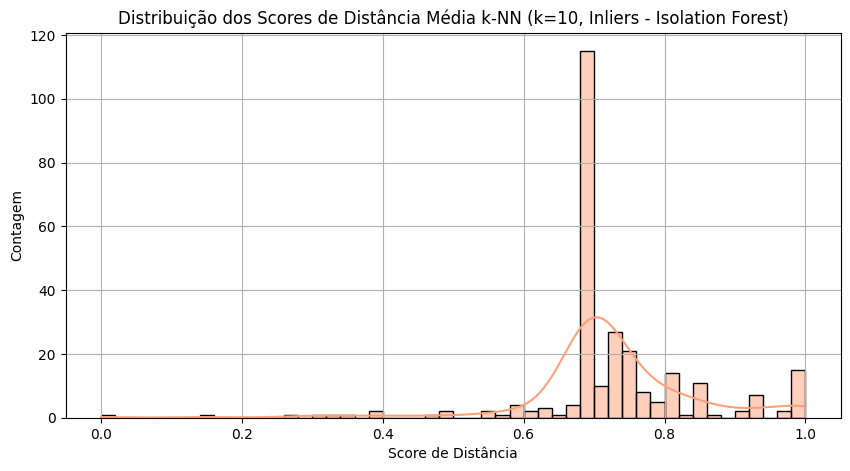
\includegraphics[width=0.9\textwidth]{imagens/swile_knn.png}
    \caption{DBS — Distribuição de Scores k-NN (Swile).}
    \label{fig:swile_knn}
    \legend{Fonte: elaboração própria.}
\end{figure}

% --- TOTALPASS ---
\subsubsection*{TotalPass}
\noindent
O centróide do TotalPass permanece bem definido e com dispersão reduzida (convergência em 0,96–0,98), enquanto o k-NN confirma proximidade local consistente, com poucas observações afastadas.

\begin{figure}[H]
    \centering
    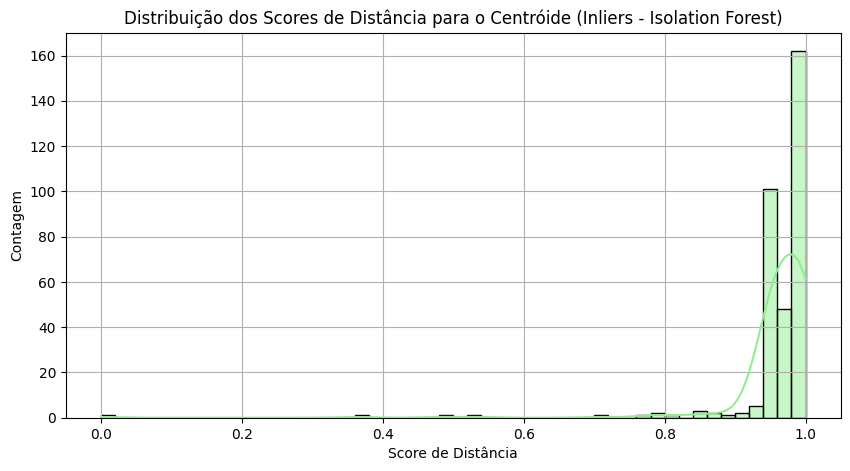
\includegraphics[width=0.9\textwidth]{imagens/totalpass_centroid.png}
    \caption{DBS — Distância ao Centróide (TotalPass).}
    \label{fig:totalpass_centroid}
    \legend{Fonte: elaboração própria.}
\end{figure}

\begin{figure}[H]
    \centering
    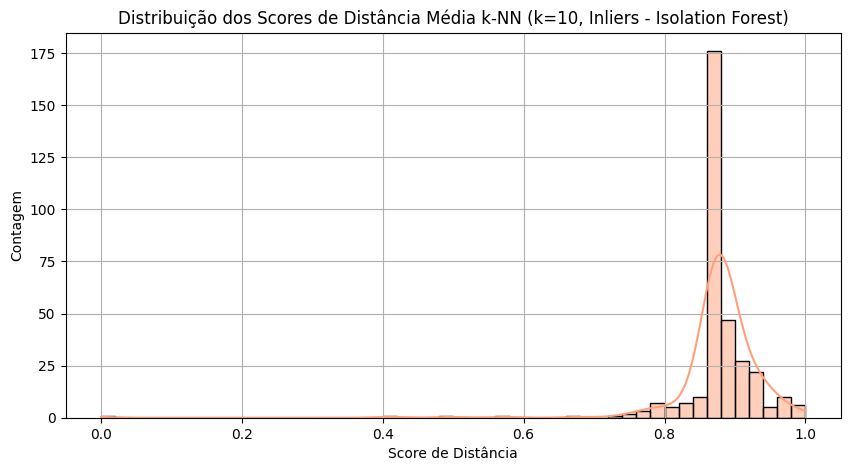
\includegraphics[width=0.9\textwidth]{imagens/totalpass_knn.png}
    \caption{DBS — Distribuição de Scores k-NN (TotalPass).}
    \label{fig:totalpass_knn}
    \legend{Fonte: elaboração própria.}
\end{figure}

% --- UNIMED ---
\subsubsection*{Unimed}
% \noindent
% A Unimed apresenta centróide com valores muito altos (≈0,98), refletindo forte similaridade global; a curva k-NN reforça a homogeneidade, com densidade concentrada e cauda curta, típica de perfis institucionais.

\begin{figure}[H]
    \centering
    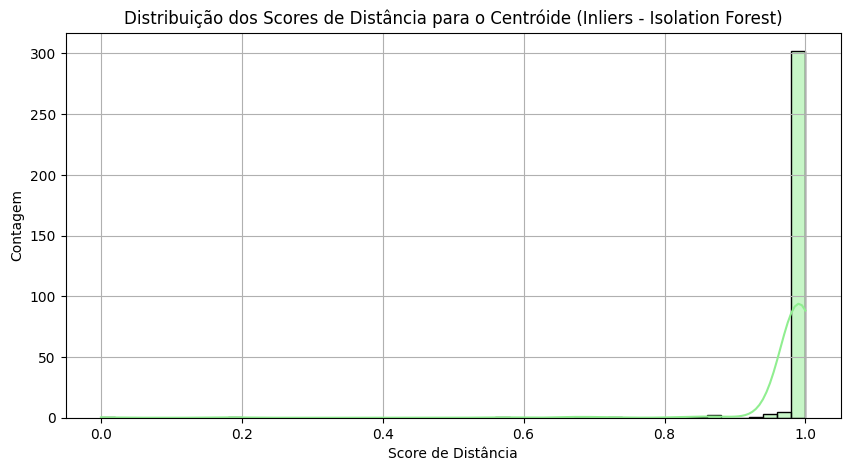
\includegraphics[width=0.9\textwidth]{imagens/unimed_centroid.png}
    \caption{DBS — Distância ao Centróide (Unimed).}
    \label{fig:unimed_centroid}
    \legend{Fonte: elaboração própria.}
\end{figure}

\begin{figure}[H]
    \centering
    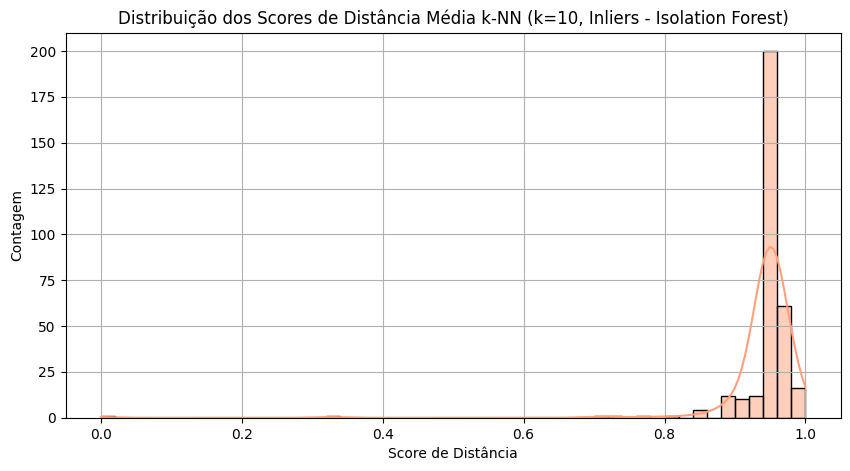
\includegraphics[width=0.9\textwidth]{imagens/unimed_knn.png}
    \caption{DBS — Distribuição de Scores k-NN (Unimed).}
    \label{fig:unimed_knn}
    \legend{Fonte: elaboração própria.}
\end{figure}

Em conjunto, os resultados do DBS reforçam a robustez e estabilidade da metodologia, uma vez que os padrões observados são consistentes entre bases distintas e mantêm alta similaridade média, independentemente do tamanho ou da composição do conjunto de empresas.

\section{Ranking Final e Ajuste de Pesos}

Após o cálculo dos scores DBS ponderados ($w_{centróide}=0{,}8$ e $w_{kNN}=0{,}2$), obteve-se o ranking final de aderência ao ICP. As Tabelas abaixo apresentam, para cada provedor, as dez empresas mais alinhadas (\textit{Top 10}) e as cinco menos alinhadas (\textit{Bottom 5}). Essa visualização permite comparar a coerência do modelo entre diferentes bases, evidenciando padrões comuns entre os ICPs.

É importante destacar que, em todos os provedores, o primeiro item do \textit{Bottom 5} apresenta score igual a zero. Esse resultado não representa necessariamente uma empresa real com desempenho nulo, mas decorre de uma condição de referência no processo de normalização e escalonamento dos scores do modelo híbrido OCC--DBS. Durante a padronização final, os valores de distância ao centróide e à vizinhança $k$ mais próxima são reescalonados para o intervalo $[0,\,1]$, de modo que o menor valor observado na amostra (empresa mais distante da região de densidade do ICP) é mapeado para zero. Assim, a pontuação mínima não implica ausência total de similaridade, mas sim o limite inferior do espaço de aderência, correspondendo ao ponto mais afastado do conjunto de empresas consideradas “normais” pelo modelo OCC. 

Em outras palavras, o score igual a zero atua como um \textit{ponto âncora} do ranqueamento, permitindo interpretar os demais valores de forma relativa — isto é, quanto mais próximo de um, maior a similaridade com o perfil ideal; quanto mais próximo de zero, maior o desvio em relação às características típicas do ICP. Esse comportamento reforça a consistência do processo de normalização, garantindo comparabilidade entre diferentes bases e assegurando que os extremos do ranqueamento representem, de fato, os limites estatísticos do modelo.


% -------- GYMPASS ---------
\begin{table}[p]
    \centering
    \caption{Ranking final de empresas para o provedor Gympass: Top 10 e Bottom 5.}
    \label{tab:7_6_ranking_gympass}
    \begin{minipage}{0.48\textwidth}
    \centering
    \textbf{Top 10 (ICP)}\\
    \begin{tabular}{p{5cm}p{1.8cm}}
    \toprule
    Empresa & Score \\
    \midrule
    Sprinklr & 0,999 \\
    Azos Labs & 0,999 \\
    DigiBee & 0,999 \\
    Hexagon & 0,999 \\
    Capco & 0,999 \\
    Rocket Lawyer & 0,999 \\
    SmartBreeder & 0,999 \\
    Linkcom & 0,999 \\
    Linx Sistemas & 0,998 \\
    CI\&T & 0,990 \\
    \bottomrule
    \end{tabular}
    \end{minipage}\hfill
    \begin{minipage}{0.48\textwidth}
    \centering
    \textbf{Bottom 5 (Outliers)}\\
    \begin{tabular}{p{5cm}p{1.8cm}}
    \toprule
    Empresa & Score \\
    \midrule
    Itaú Unibanco & 0,000 \\
    Tata Consultancy Services & 0,047 \\
    Deloitte & 0,338 \\
    Ambev & 0,385 \\
    DHL & 0,079 \\
    \bottomrule
    \end{tabular}
    \end{minipage}
\end{table}
% -------- PSICOLOGIA VIVA ---------
\begin{table}[p]
    \centering
    \caption{Ranking final de empresas para o provedor Psicologia Viva: Top 10 e Bottom 5.}
    \label{tab:7_6_ranking_psicologiaviva}
    \begin{minipage}{0.48\textwidth}
    \centering
    \textbf{Top 10 (ICP)}\\
    \begin{tabular}{p{5cm}p{1.8cm}}
    \toprule
    Empresa & Score \\
    \midrule
    Barbosa Supermercados & 0,9996 \\
    Avenida & 0,9995 \\
    SRM ASSET & 0,9988 \\
    Escola Villare & 0,9988 \\
    Docket & 0,9981 \\
    Procfit & 0,9980 \\
    ROIT & 0,9980 \\
    Empório Alex & 0,9978 \\
    Laboratório Fantasma & 0,9977 \\
    Rock Encantech & 0,9965 \\
    \bottomrule
    \end{tabular}
    \end{minipage}\hfill
    \begin{minipage}{0.48\textwidth}
    \centering
    \textbf{Bottom 5 (Outliers)}\\
    \begin{tabular}{p{5cm}p{1.8cm}}
    \toprule
    Empresa & Score \\
    \midrule
    Banco Bradesco & 0,0000 \\
    EY & 0,093 \\
    Atento & 0,836 \\
    Atacadão & 0,842 \\
    Localiza\&Co & 0,858 \\
    \bottomrule
    \end{tabular}
    \end{minipage}
\end{table}
% -------- SWILE ---------
\begin{table}[p]
    \centering
    \caption{Ranking final de empresas para o provedor Swile: Top 10 e Bottom 5.}
    \label{tab:7_7_ranking_swile}
    \begin{minipage}{0.48\textwidth}
    \centering
    \textbf{Top 10 (ICP)}\\
    \begin{tabular}{p{5cm}p{1.8cm}}
    \toprule
    Empresa & Score \\
    \midrule
    BYX & 0,9987 \\
    Certsys & 0,9987 \\
    Tax.Co & 0,9987 \\
    Sem nome & 0,9987 \\
    Vai Voando & 0,9986 \\
    Better Now & 0,9985 \\
    Fluencypass & 0,9985 \\
    Construmarket & 0,9985 \\
    NaN & 0,9984 \\
    Empiricus & 0,9983 \\
    \bottomrule
    \end{tabular}
    \end{minipage}\hfill
    \begin{minipage}{0.48\textwidth}
    \centering
    \textbf{Bottom 5 (Outliers)}\\
    \begin{tabular}{p{5cm}p{1.8cm}}
    \toprule
    Empresa & Score \\
    \midrule
    Brisanet Telecomunicações & 0,0000 \\
    Reply & 0,208 \\
    Mitre Realty & 0,345 \\
    Softtek & 0,359 \\
    Egis & 0,398 \\
    \bottomrule
    \end{tabular}
    \end{minipage}
\end{table}
% -------- TOTALPASS ---------
\begin{table}[!htbp]
    \centering
    \caption{Ranking final de empresas para o provedor TotalPass: Top 10 e Bottom 5.}
    \label{tab:7_6_ranking_totalpass}
    \begin{minipage}{0.48\textwidth}
    \centering
    \textbf{Top 10 (ICP)}\\
    \begin{tabular}{p{5cm}p{1.8cm}}
    \toprule
    Empresa & Score \\
    \midrule
    GoodStorage & 0,999 \\
    Safira Holding & 0,999 \\
    Sou SERAC & 0,999 \\
    minu.co & 0,999 \\
    Simpar & 0,999 \\
    Rede Ápice & 0,998 \\
    JHSF Participações & 0,993 \\
    Ilia Digital & 0,991 \\
    Intelipost & 0,991 \\
    Leega Consultoria & 0,991 \\
    \bottomrule
    \end{tabular}
    \end{minipage}\hfill
    \begin{minipage}{0.48\textwidth}
    \centering
    \textbf{Bottom 5 (Outliers)}\\
    \begin{tabular}{p{5cm}p{1.8cm}}
    \toprule
    Empresa & Score \\
    \midrule
    JBS & 0,000 \\
    Atacadão & 0,372 \\
    Gerdau & 0,484 \\
    Dasa & 0,543 \\
    Hospital Albert Einstein & 0,699 \\
    \bottomrule
    \end{tabular}
    \end{minipage}
\end{table}
% -------- UNIMED ---------
\begin{table}[!htbp]
    \centering
    \caption{Ranking final de empresas para o provedor Unimed: Top 10 e Bottom 5.}
    \label{tab:7_5_ranking_unimed}
    \begin{minipage}{0.48\textwidth}
    \centering
    \textbf{Top 10 (ICP)}\\
    \begin{tabular}{p{5cm}p{1.8cm}}
    \toprule
    Empresa & Score \\
    \midrule
    MaisTODOS & 0,9992 \\
    Internet Way\textregistered & 0,9992 \\
    ENELO & 0,9990 \\
    Basecol Mix & 0,9989 \\
    Solinftec & 0,9988 \\
    SGF Global & 0,9956 \\
    Qive & 0,9952 \\
    Cimoagro & 0,9950 \\
    Shift & 0,9950 \\
    Corebiz & 0,9949 \\
    \bottomrule
    \end{tabular}
    \end{minipage}\hfill
    \begin{minipage}{0.48\textwidth}
    \centering
    \textbf{Bottom 5 (Outliers)}\\
    \begin{tabular}{p{5cm}p{1.8cm}}
    \toprule
    Empresa & Score \\
    \midrule
    Atacadão & 0,0000 \\
    Continental & 0,212 \\
    Sherwin-Williams & 0,593 \\
    Riachuelo & 0,689 \\
    thyssenkrupp & 0,690 \\
    \bottomrule
    \end{tabular}
    \end{minipage}
\end{table}

\FloatBarrier % <- garante que as tabelas sejam posicionadas antes do próximo texto

Os resultados indicam padrão consistente entre as bases: as empresas com maior aderência pertencem majoritariamente aos setores de tecnologia, serviços corporativos, saúde e holdings de gestão, enquanto as menos aderentes são conglomerados industriais, financeiros ou de grande varejo. A manutenção de uma estrutura de ranking similar entre bases distintas reforça a estabilidade do modelo híbrido proposto.

% \section{Visualizações e Explicabilidade do Modelo}

% A projeção PCA (Figura~\ref{fig:7_6_pca}) mostra um agrupamento central composto por empresas de alto score, enquanto os outliers aparecem dispersos nas bordas do plano. Já o boxplot (Figura~\ref{fig:7_7_box}) evidencia que empresas com número de funcionários entre 100 e 1.000 concentram os maiores scores finais.

% % Inserir Figura 7.6 — PCA colorido por score final
% % Inserir Figura 7.7 — Boxplot de funcionários por faixa de score

% \section{Discussão Integrada dos Resultados}

% Os resultados confirmam a efetividade do modelo híbrido em identificar o perfil ideal de cliente (ICP) da TotalPass. O baixo número de anomalias (5\% da base) e as médias elevadas dos scores DBS indicam que a maioria das empresas compartilha características firmográficas comuns. O ICP identificado concentra-se em empresas de médio porte, capital consolidado e atuação em setores tecnológicos e de serviços.

% \section{Considerações Finais do Capítulo}

% O estudo de caso da TotalPass demonstrou a consistência da abordagem OCC + DBS na definição de ICPs. Nas próximas iterações, os mesmos procedimentos serão aplicados às bases da Gympass, Swile, Unimed e Psicologia Viva, possibilitando comparações cruzadas e avaliação da robustez do modelo frente a diferentes perfis de negócio.

\include{capitulos/Conclusão}

\begin{thebibliography}{99}

\bibitem[Seliya et al.(2021)]{Seliya2021} SELIYA, Naresh; KUMAR, Vivek; KANCHAN, Ankit. 
\textbf{A review of one-class classification: Applications and challenges}. 
Applied Intelligence, v. 51, n. 2, p. 1–23, 2021. 
DOI: \url{https://doi.org/10.1007/s10489-020-01838-3}.

\bibitem[Wu et al.(2023)]{Wu2023} WU, X.; ZHANG, Y.; LI, H. 
\textbf{A comprehensive survey on lead scoring models in B2B marketing}. 
Journal of Business Research, v. 160, p. 113–128, 2023. 
DOI: \url{https://doi.org/10.1016/j.jbusres.2023.113128}.

\bibitem[Nygård(2020)]{Nygard2020} NYGÅRD, Magnus. 
\textbf{Automating lead scoring with machine learning: A case study}. 
Master’s Thesis — Norwegian University of Science and Technology, Trondheim, 2020.

\bibitem[Qian et al.(2019)]{Qian2019} QIAN, Kun; ZHOU, Li; WANG, Rui. 
\textbf{Distance-based ranking models for customer prioritization}. 
Expert Systems with Applications, v. 127, p. 144–156, 2019. 
DOI: \url{https://doi.org/10.1016/j.eswa.2019.02.038}.

\bibitem[Mancisidor et al.(2018)]{Mancisidor2018} MANCISIDOR, Andrés; RIVERA, Antonio; GARCÍA, David. 
\textbf{Customer segmentation using autoencoders and classification methods}. 
Procedia Computer Science, v. 144, p. 51–59, 2018. 
DOI: \url{https://doi.org/10.1016/j.procs.2018.10.488}.

\bibitem[Golbayani, Florescu e Chatterjee(2020)]{Golbayani2020} GOLBAYANI, Parham; FLORESCU, Laura; CHATTERJEE, Samir. 
\textbf{A comparative study of forecasting corporate credit ratings using Neural Networks, SVM, and Decision Trees}. 
Expert Systems with Applications, v. 142, p. 112–124, 2020. 
DOI: \url{https://doi.org/10.1016/j.eswa.2020.112124}.

% ---------- Referências complementares (citadas no texto) ----------

\bibitem[Pono(2020)]{Pono2020} PONO. 
\textbf{Ideal Customer Profile: How to define your perfect B2B customer}. 
Pono Consulting, 2020. 
Disponível em: \url{https://pono.io/blog/ideal-customer-profile}. 
Acesso em: 5 nov. 2025.

\bibitem[Experian(2020)]{Experian2020} EXPERIAN. 
\textbf{B2B data quality trends and best practices}. 
Experian Global Data Report, 2020. 
Disponível em: \url{https://www.experian.com/business}. 
Acesso em: 5 nov. 2025.

\bibitem[Inflexion-Point(2020)]{Inflexion2020} INFLEXION-POINT STRATEGY PARTNERS. 
\textbf{Understanding your ideal customer profile}. 
Inflexion-Point White Paper, 2020. 
Disponível em: \url{https://www.inflexion-point.com}. 
Acesso em: 5 nov. 2025.

\bibitem[McKinsey(2020)]{McKinsey2020} McKINSEY \& COMPANY. 
\textbf{Data-driven marketing and sales: Redefining customer engagement in B2B}. 
McKinsey Insights, 2020. 
Disponível em: \url{https://www.mckinsey.com}. 
Acesso em: 5 nov. 2025.

\bibitem[TOPO(2020)]{TOPO2020} TOPO. 
\textbf{The state of lead management and ICP definition}. 
TOPO Research Report, 2020. 
Disponível em: \url{https://www.topohq.com}. 
Acesso em: 5 nov. 2025.

\bibitem[BRASIL(2018)]{Brasil2018} BRASIL. 
\textbf{Lei nº 13.709, de 14 de agosto de 2018}. 
Lei Geral de Proteção de Dados Pessoais (LGPD). 
\textit{Diário Oficial da União}, Brasília, DF, 15 ago. 2018.

\bibitem[IBGE(2020)]{IBGE2020} INSTITUTO BRASILEIRO DE GEOGRAFIA E ESTATÍSTICA (IBGE). 
\textbf{Classificação Nacional de Atividades Econômicas – CNAE 2.3}. 
Rio de Janeiro: IBGE, 2020. 
Disponível em: \url{https://www.ibge.gov.br}. 
Acesso em: 5 nov. 2025.

\bibitem[ReceitaFederal(2020)]{Receita2020} RECEITA FEDERAL DO BRASIL. 
\textbf{Cadastro Nacional da Pessoa Jurídica (CNPJ)}. 
Brasília: Ministério da Fazenda, 2020. 
Disponível em: \url{https://www.gov.br/receitafederal}. 
Acesso em: 5 nov. 2025.

\bibitem[LinkedIn(2025)]{LinkedIn2025} LINKEDIN CORPORATION. 
\textbf{LinkedIn Company Data API}. 
Disponível em: \url{https://developer.linkedin.com}. 
Acesso em: 5 nov. 2025.

\end{thebibliography}


\end{document}

